\documentclass[./../../paper.tex]{subfiles}
\graphicspath{{\subfix{./../../figures/}}}

\begin{document}
Many processes, often medical, economical, or administrative in nature, are governed by sequential events and their contextual environment. Many of these events and their order of appearance play a crucial part in the determination of every possible outcome\cite{vanderaalst_ProcessMiningManifesto_2012}. With the rise of AI and the increased abundance of data in recent years, several techniques emerged that help to predict the outcomes of complex processes in the real world. A field that focuses on modelling processes is \gls{PM}.

Research in the Process Mining discipline has shown that it is possible to predict the outcome of a particular process fairly well\cite{tax_PredictiveBusinessProcess_2017a,klimek_Longtermseriesforecasting_2021}.

For instance, in the medical domain, models have been shown to predict the outcome or trajectory of a patient's condition\cite{mannhardt_Analyzingtrajectoriespatients_2017}. In the private sector, process models can be used to detect faults or outliers. The research discipline \gls{DL} has shown promising results within domains that have been considered difficult for decades. The Moravex Paradox\cite{agrawal_studyphenomenonMoravec_2010}, which postulates that machines are capable of doing complex computations easily while failing in tasks that seem easy to humans such as object detection or language comprehension, does not hold anymore. Meaning that with enough data to learn, machines are capable of learning highly sophisticated tasks better than any human. The same holds for predictive tasks. However, while many prediction models can predict certain outcomes, it remains a difficult challenge to understand their reasoning. 

This difficulty arises from models, like neural networks, that are so-called \emph{\glspl{bbm}}. Meaning, that their inference is incomprehensible, due to the vast amount of parameters involved. This lack of comprehension is undesirable for many fields like IT or finance. Not knowing why a loan was given, makes it impossible to rule out possible biases. Knowing what will lead to a system failure will help us knowing how to avoid it. In critical domains like medicine, the reasoning behind decisions becomes crucial. For instance, if we know that a treatment process of a patient reduces the chances for survival, we want to know which treatment step is the critical factor we ought to avoid. To summarise, knowing the outcome of a process often leads us to questions on how to change it. Formally, we want to change the outcome of a process instance by making it maximally likely with as little interventions as possible\cite{molnar2019}. \autoref{fig:desired_outcome} is a visual representation of the desired goal.

\begin{figure}[htb]
    \centering
    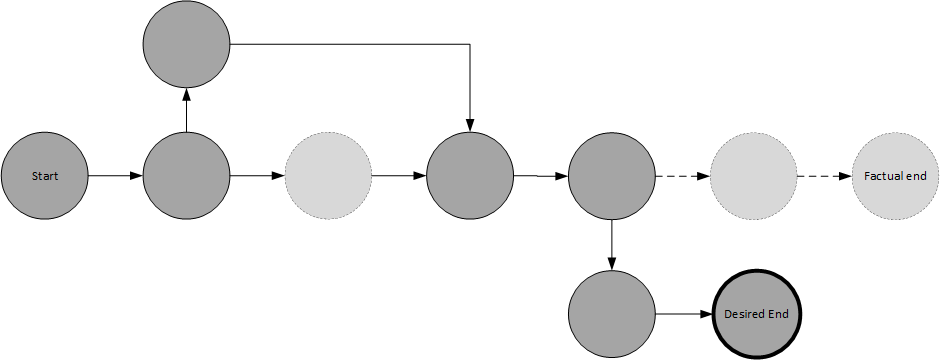
\includegraphics[width=0.99\textwidth]{figures/counterfactual_goal.png}
    \caption{This figure illustrates a model, that predicts a certain trajectory of the process. However, we want to change the process steps in such a way, that it changes the outcome.}
    \label{fig:desired_outcome}
\end{figure}

\noindent One way to better understand the \gls{ML} models lies within the \gls{XAI} discipline. XAI focuses the developments of theories, methods, and techniques that help explaining \glspl{bbm} models to humans. Most of the discipline's techniques produce explanations that guide our understanding. Explanations can come in various forms, such as IF-THEN rules\cite[p.90]{molnar2019} or feature importance\cite[p.45]{molnar2019}, but some are more comprehensible for humans than others. 

A prominent and human-friendly approach are \emph{counterfactuals}\cite[p. 221]{molnar2019}. Counterfactuals within the AI framework help us to answer hypothetical "what-if" questions. Basically, if we know \emph{what} would happen \emph{if} we changed the execution of a process instance, we could change it for the better. In this thesis, we raise the question how we can use counterfactuals to change the trajectory of a process models' prediction towards a desired outcome. Knowing the answers not only increases the understanding of \glspl{bbm}, but also help us avoid or enforce certain outcomes. 
\end{document}